\documentclass[fypca]{socreport}

\usepackage{fullpage}
\usepackage{float}
\usepackage{hyperref}
\usepackage{graphicx}
\usepackage[shortlabels]{enumitem}
\usepackage[utf8]{inputenc}
\graphicspath{{./figs/}}

%%% Begin document
\begin{document}
\pagenumbering{roman}
\title{Underwater Real-Time Object Recognition and Tracking for Autonomous Underwater Vehicle}
\author{Tan Soon Jin}
\projyear{2016/17}
\projnumber{H021400}
\advisor{Prof. Terrence Sim Mong Cheng}
\deliverables{
    \item Report: 1 Volume}

\maketitle

\begin{abstract}
This project proposes and implements a near real-time vision processing framework on the \textit{Bumblebee AUV (Autonomous Underwater Vehicle)} that participates in Robosub, an international autonomous robotics submarines held annually in San Diego hosted by AUVSI (Association for Unmanned Vehicle Systems International).

The implemented vision system will be deployed on the AUV to complete a series of visual tasks during the competition that mimics real world underwater application such as collecting data on marine life-forms, repairing underwater pipeline etc. Though there are many state-of-the-art vision algorithms developed by the community, the underwater domain poses an entirely different set of challenges such as low contrast, color degradation and underwater perturbations that demands a different vision processing approach.

The primary contribution of the project is to implement a vision framework consisting of a set of modular vision modules and pipelines for real-time object tracking in different underwater conditions. It is essential that the the vision framework is both a) adaptive, b) robust and c) easy to use. With the implemented vision modules, the project's secondary contribution aims to automate parameter selection and model selection; taking the human out of the loop.

\begin{descriptors}
    \item Computer System Implementation
    \item Visual Computing
\end{descriptors}
\begin{implement}
    Python, ROS (Robot Operating System)
\end{implement}
\end{abstract}

\begin{acknowledgement}
    I would like to acknowledge the advice and guidance by my supervisor Prof. Terrence Sim Mong Cheng in this project.
\end{acknowledgement}


\listoffigures
\listoftables

%%%%%%%%%%%%%%%%%%%%%%%%%%%%%%%%%%%%%%%%%%%%%%%%%%%%%%%%%%%%%%%%%%%%%%%%%%%%%%%
% Chapter 1
%%%%%%%%%%%%%%%%%%%%%%%%%%%%%%%%%%%%%%%%%%%%%%%%%%%%%%%%%%%%%%%%%%%%%%%%%%%%%%%

\chapter{Introduction}

\section{Background on Robosub}

\subsection{Information about the competition}
Robosub is an international AUV competition where students from around
the world build their own customized AUV to complete a series of
underwater missions that involve both visual tasks and acoustics task.
The competition is held annually in TRANSDEC (Transducer Evaluation
Center) man-made pool.

\begin{figure}[ht]
\centering

        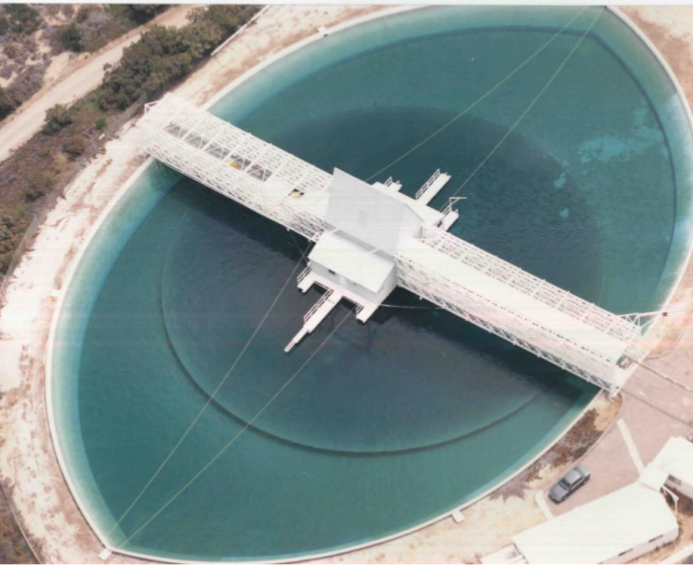
\includegraphics[width=0.8\textwidth, height=0.3\textheight]{transdec_aerial.png}
        \caption{Aerial view of TRANSDEC. Operational depth of 16 ft for most vision tasks}
        \label{fig:transdec_aerial}

\end{figure}

\subsection{Description of vision tasks}
Vision tasks in Robosub can divided into forward-facing tasks and
bottom-facing tasks which poses different sets of challenges. Since the
tasks do not vary significantly every year, we can use datasets
collected from this year's competition as testbed for our vision
algorithms.

\begin{figure}[ht]
\centering

        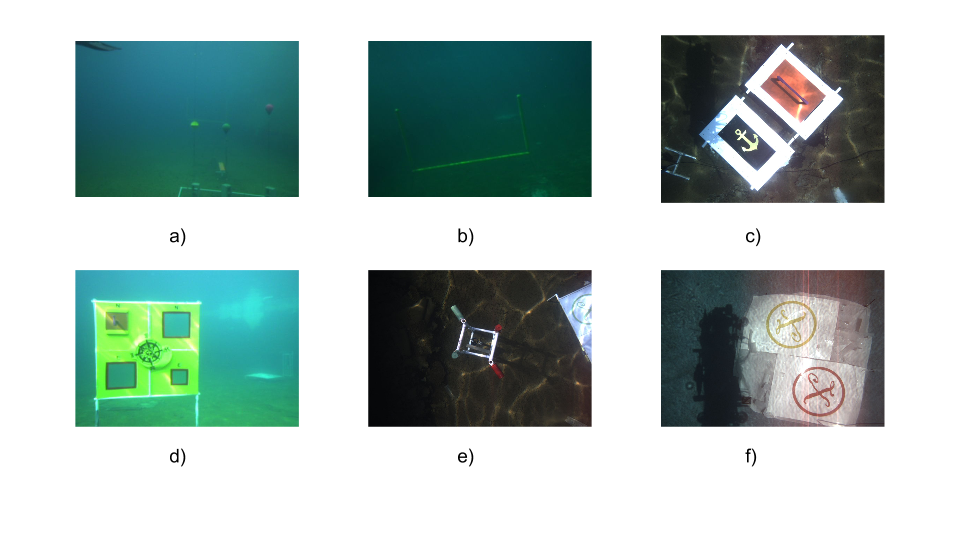
\includegraphics[width=0.8\textwidth, height=0.3\textheight]{robosub_vision_tasks.png}
        \caption{Robosub 2016 Vision Tasks. a) Scuttle Ship b) Navigate
        Channel c) Weigh Anchor d) Set Course e) Bury Treasure (Coins)
        f) Bury Treasure (Island)}
        \label{fig:robosub2016_tasks}

\end{figure}

\begin{enumerate}
    \item \textbf{Scuttle Ship (Buoy)}
        A recurring task where the AUV has identify the correct color
        buoy and touch it. There are two major challenges with this
        task:
        \begin{enumerate}[a.]
        \item Red buoy tends to exhibit color distortion as red
          wavelength attenuates the fastest \cite{Galdran2015}.
        \item Non-uniform illumination on top-half of buoys make it hard
          to distinguish the buoys.
        \end{enumerate}
    \item \textbf{Navigate Channel} \\
        The AUV is required to move in between and over the PVC pipes.
    \item \textbf{Weight Anchor} \\
        Classic object classification task where the AUV is required to
        drop a marker into the correct bin to obtain maximum points
        after removing the cover using a manipulator.
    \item \textbf{Set Course} \\
        Identification of covered square (orange panel) and remove it.
        Fire two markers over 2 smaller holes. As yellow and orange are
        really close on the colour spectrum, this forces us to use other
        visual cues such as edge for better detection.
    \item \textbf{Bury Treasure} \\
        For this task, one has to identify the small cylinders (red and
        green) and drop them onto their respective colored circles (on
        the Island). Identifying and distinguishing small objects afar
        (4 m) underwater is the biggest challenge in this task. Besides
        that, the dropped cylinders may potentially occlude the circles.
\end{enumerate}

\section{Challenges in Underwater Image Processing}

Many literature such as \outcite{M2016} that investigates various
underwater image restoration methods cite haze formation which happens
as light propagated from object undergoes attenuation and scattering
causing image with low contrast. In addition, Beer-Lambert law
\cite{gevers2012color} states relates attenuation of light to properties
of water medium; therefore, light components with low wavelength; green
and blue are not as easily absorbed compared to red wavelength. This
causes underwater images tend to have greenish or bluish color cast.

\begin{figure}[ht]
\centering

        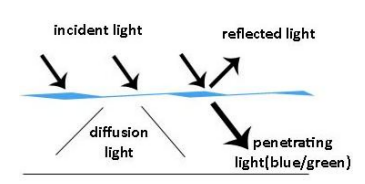
\includegraphics[width=0.8\textwidth, height=0.2\textheight]{underwater_beerlambert.png}
        \caption{Absorption of light at the surface}
        \label{fig:water_surface_effect}

\end{figure}

\section{Project Requirements Analysis}
Though it is the objective of the project to design a vision framework
for the Robosub missions, the vision framework should also be easily
extended to work for more complex real world applications. 

\subsection{Nature of tasks}
\begin{enumerate}
    \item Vision algorithms perform with acceptable accuracy under the following conditions:
    \begin{figure}[ht]
    \centering
            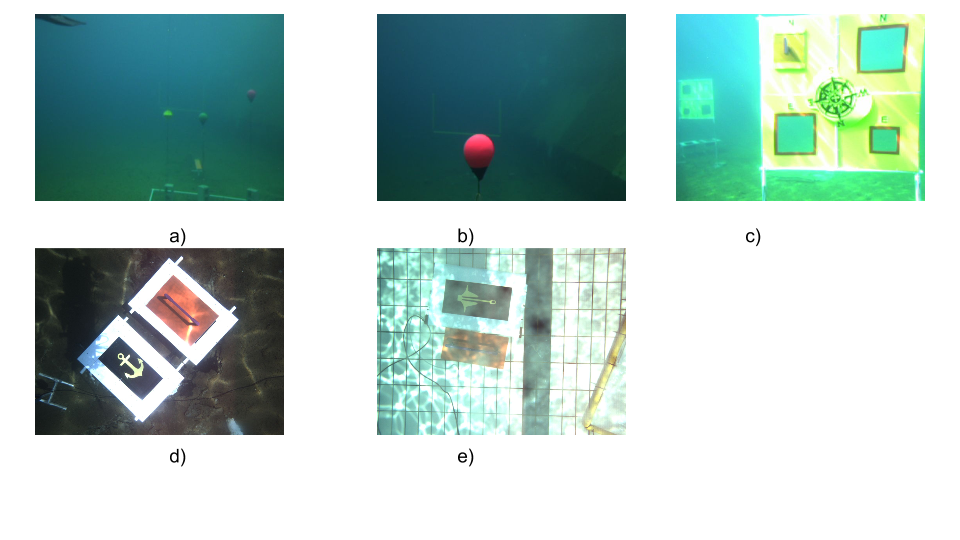
\includegraphics[width=0.8\textwidth, height=0.3\textheight]{task_challenges.png}
            \caption{Different vision challenges. a) Haze formation b)
            Partial occlusion c) Non-uniform illumination d) Sunlight
            flickers e) Shadow}
            \label{fig:vision_challenges}
    \end{figure}
    \item Low detection latency (near real-time) \\
        AUV needs to make swift decision based on sensor inputs to
        complete task under time constraints (same for real world time
        critical mission i.e underwater mine detection)
    \item Geometric properties of objects are made known in advance
    \item Short-period single target tracking for  task (unlike video surveillance application)
    \item Able to detect objects from far away (5m) and near distance (for manipulation task)
\end{enumerate}

%%%%%%%%%%%%%%%%%%%%%%%%%%%%%%%%%%%%%%%%%%%%%%%%%%%%%%%%%%%%%%%%%%%%%%%%%%%%%%%
% Chapter 2
%%%%%%%%%%%%%%%%%%%%%%%%%%%%%%%%%%%%%%%%%%%%%%%%%%%%%%%%%%%%%%%%%%%%%%%%%%%%%%%

\chapter{Literature Review}
This review is conducted with the purpose to investigate and select most
suitable algorithms that generate the best result on the Robosub
datasets. Since every teams who participate in Robosub are required to
submit a journal paper,vision algorithms deployed by top-peforming
schools such as Cornell University, University of Florida and École de
technologie supérieure provide valuable insights on image processing
that are effective in underwater environment. Besides that, review of
popular image processing techniques in particular on topics like object
detection, object tracking, color constancy, saliency mechanism,
detection proposals and adapatation of algorithms.

\section{Preprocessing}
\subsection{Underwater Image Enhancement}
The paper by \outcite{garcia2002way} compared methods such as
homomorphic filtering and local adaptive histogram equalization
(Contrast Limited Adaptive Histogram) which considers that image is a
product of illumination and reflectance properties. However, homomorphic
filter has the benefit of preserving sharp edges while attenuating
non-uniform illumination. On the other hand, by only redistributing
pixels exceeding a clipping level to increase contrast of an image,
CLAHE manages to reduce noise amplification in normal local histogram
equalization.

Instead of relying on a single image, \outcite{Gracias2008} recover
corrupted underwater image by finding the difference between the current
frame with temporal median of a registered set of N frames. Image
dehazing is equally as important to ensure good performance of further
image processing operation such feature detection. \outcite{Kaiming2011}
proposed a single image dehazing method using the dark channel prior
which states that haze-free image contains local region with low
intensities in at least one color channel. \outcite{Galdran2015} propose
a variant of dark channel prior for underwater environment, the Red
Channel method as red color shows most degradation in turbid water
medium. From another perspective, \outcite{Ancuti2011} takes a
fusion-approach to recover the original image by generating a few weight
maps that correlates with intrinsic properties of the image itself. A
color corrected and contrast enhanced of the input image are used to
generate different weight maps that are fused using a Laplacian
multi-scale strategy to generate a smoothed output image. This method
has the benefit of using a single image but the weight maps must be
combined with different weightage to achieve an ideal result. 

\subsection{Color Constancy}
Color cue plays an important role to distinguish different objects such
as the small cylinders in Robosub that requires sorting by color. The
ability to account for color of the light source is called color
constancy. The work of \outcite{Gijsenij2011} analyzes various color
constancy algorithms. Attention is paid especially on low-level
statistics methods that are computationally inexpensive compared to
learning-based methods. The Grey-World \cite{buchsbaum1980spatial}
estimate the color of the light source by estimating the average color
in the image assuming that any deviation from average color (Grey) is
caused by illuminants. The White-Patch method \cite{land1977retinex}
estimates the color of light source by computing the maximum response in
individual RGB color channels. \outcite{finlayson2004shades} shows that
both Grey-World and White-Patch algorithms are special instantiation of
a more general color constancy algorithm based on Minkowski norm called
Shades of Grey. Their investigation of best illumination estimation
suggests using Minkowski norm, p = 6 to obtain optimal performance.

Though we see new method such as the Color Rabbit \cite{Bani??2014}
which combine multiple local illumination estimations to a global one,
these class of methods are more computationally expensive which is not
suitable for real-time application. Inspired by primary visual cortex
(V1) of human visual system (HVS), \outcite{Gao2013} estimate the true
illuminant color of a scene by computing the maximum response in
separate RGB channels of the responses of double-opponent cells. This
method is shown to perform better on outdoor scenes from Gehler-Shi
dataset where the mean reflectance is not achromatic which is assumed by
Grey-World based methods. 

\section{Saliency Region Detection}
Ability of human visual system (HVS) to selectively process only the
salient visual stimuli, specifically salient object detection helps to
reduce computation time of object recognition that traditionally relies
of sliding-window approach to detect object of interest.
\outcite{achanta2009frequency} estimate centre-surround contrast using
color and luminance features using a frequency-tuned approach to
generate high-resolution saliency map. In contrast, biological inspired
method of \cite{Itti1998} that computes centre-surround contrast using
Difference of Gaussian (DoG) which generates low resolution map and
ill-defined boundaries because of down sampling of original
image.Because saliency detection often work poorly in low contrast
environment i.e underwater environment, work of
\outcite{VanDeWeijer2005} boost local color information by analyzing
isosalient colour derivatives. \outcite{Cao2010} extended work of Van de
Weijer as Gaussian derivatives of each opponent color to get a better
iso-salient transformation. 

\section{Detection Proposals}
Relying on saliency mechanism is insufficient in perturbed underwater
condition; therefore, different detection proposals algorithms are
investigated. \outcite{Hosang2015} cited that "detection proposals"
which can be grouped into a) grouping proposal methods and b) Window
scoring proposals methods are used extensively by top performing object
detectors in PASCAL and ImageNet. On top of reduced computation cost by
avoiding exhaustive sliding window approach, detection proposals improve
recall by filtering out false positives. Recent work of
\outcite{Winschel2016} combines top performing detection proposals
methods, SelectiveSearch \cite{uijlings2013selective} and EdgeBox
\cite{zitnick2014edge}. Though detection proposals allow for faster
object recognition, it is important that it does not filter out object
of interest and incur more computation costs that out weights time
saved.

\section{Object Detection and Tracking}
An overall review of journal papers submitted by top-performing teams in
Robosub shows a general trend of combining surprisingly simple computer
vision techniques such as adaptive color thresholding, edge detection
i.e Canny Edge \cite{canny1986computational}, and contour analysis i.e
Hu moment \cite{hu1962visual}. Team CUAUV (Cornell AUV) proposes
adaptive color thresholding on different color spaces such as LAB, LUV
and YCrCb where the individual masks are combined to form final
binarized mask. This is a blob-based detection approach where contour
generated by OpenCV's implementation of  \cite{suzuki1985topological}
will be matched against known geometric properties of desired object of
interest. \outcite{Walters2014} use particle filter approach to detect
and track object of interest. Known for its ability to deal with
non-linear noise and multi-modal hypotheses
\cite{isard1998condensation}, particle filter has the ability to recover
from wrongly tracked objects. Though more sophisticated techniques such
as neural-network classification is deployed, teams still generally rely
on low-level visual cues such as color and edge. This may be attributed
to simplicity and efficiency of mentioned algorithms.
\outcite{Benoit2014} focuses on developing sophisticated vision tuning
client that allows for rapid prototyping via "mix and match" approach to
design a suitable vision pipeline for each individual vision tasks.

%%%%%%%%%%%%%%%%%%%%%%%%%%%%%%%%%%%%%%%%%%%%%%%%%%%%%%%%%%%%%%%%%%%%%%%%%%%%%%%
% Chapter 3: Design & Methodology
%%%%%%%%%%%%%%%%%%%%%%%%%%%%%%%%%%%%%%%%%%%%%%%%%%%%%%%%%%%%%%%%%%%%%%%%%%%%%%%

\chapter{Design \& Methodology}

\section{Proposed design}

Though many solutions to underwater vision challenges exist, many of them are
not designed to work with each other as they do not share a common interface. To
increase ease of use and productivity of developers, this paper proposed a
vision framework that consists of modular components tailored for underwater
application, and ease of integration to Robot Operating System (ROS) which are
commonly used by the robotics community.

The proposed vision framework is divided into \textit{offline} modules and
\textit{online} modules. \textit{Offline} modules refer to modules that will
deployed prior to object tracking mission such as video annotation, visual data
analysis and model learning. In contrast, \textit{Online} modules are deployed
during mission such as preprocessing, object detection and object tracking.

\begin{figure}[H]
\centering
  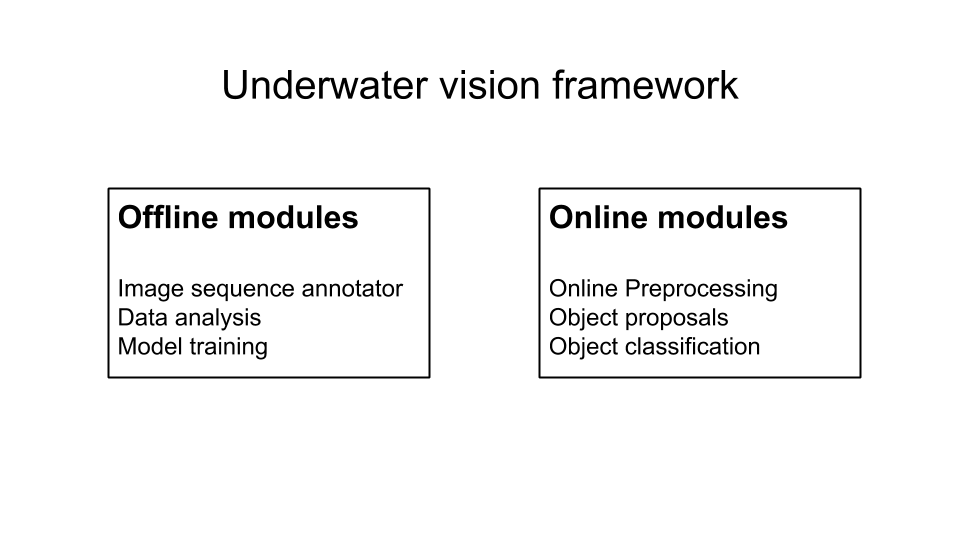
\includegraphics[width=0.8\textwidth, height=0.3\textheight]{framework.png}
  \caption{Proposed vision framework}
  \label{fig:proposed_vision_framework}
\end{figure}

\subsection{Offline modules}

\textbf{Video annotation} is extremely important for ground truth
generation that is essential for model learning. To achieve rapid ground truth
generation with limited manpower and time, model-free tracking method such as
mean-shift by (\outcite{comaniciu2002mean}) and correlation-filter based tracking
(\outcite{bolme2010visual}). Of course this is under the assumption that some
degree of localization error is acceptable and human intervention is used to
redefine the target window if drift occurs. This enables a faster testing
iteration as data collected can be integrated more quickly to update our model.

\textbf{Data analysis} helps us discover patterns and statistical nature of
collected visual data which is important for feature engineering and model
learning. These tools include visualization of image under different color
spaces, estimation of illuminants, saliency map generation and image quality
assessments. This information is used as metadata to label and categorize
dataset to increase productivity of model training and validation. Again, this
is an attempt to automate trivial task that require human attention.

\textbf{Model Training} is divided into several stages such as feature
selection, model selection and hyperparameters optimization. To increase
usability of the software without machine learning knowledge, this paper adopt the trending
automatic machine learning approach by leveraging on available open-source
libraries such as \href{https://github.com/automl/auto-sklearn}{Auto-Sklearn},
\href{https://github.com/rhiever/tpot}{TPOT}, and \href{https://github.com/automl/HPOlib}{HPOlib}.

\subsection{Online modules}

\textbf{Preprocessing} has considerable effect on accuracy of underwater object
detection because of the challenges mentioned. Color normalization is performed
on image to remove effect of color cast because of light attenuation. Low-level
stastical methods have been explored because they are simple to implement and
fast while producing accuracy comparable to other methods such as gamut mapping
and learning methods \outcite{Gijsenij2011}. In addition, fusion-based
underwater image enhancement by \outcite{fang2013effective} is implemented to
remove haze effect because of back-scattering of light. Following that, various
illumination compensation methods are executed to reduce effect of flickering and
adjusting brightness of the image for more optimal object detection.

\textbf{Object Tracking} is separated into 3 components: a) \textit{object
  proposal}, b) \textit{object classification} and c) \textit{model update}. An
adaptive object model and pre-learned object model are applied to achieve higher
tracking accuracy. \textit{Object proposals} based on superpixel, edge-detection
and saliency are exploited to produce candidates for classification instead of
the traditional sliding-window approach which is more computationally expensive.
For \textit{object classification} of candidate windows, Support Vector Machine
(SVM), Random Forest and Gaussian Process are the supported classifiers.
To improve generalization of the tracker to different conditions, a
\textit{model update} inspired by \outcite{grabner2006real} is adopted in our approach.

\newpage
\section{Methodology}

In this section we will explain how these modular components are used together
for underwater real-time object tracking.

\begin{figure}[H]
\centering
  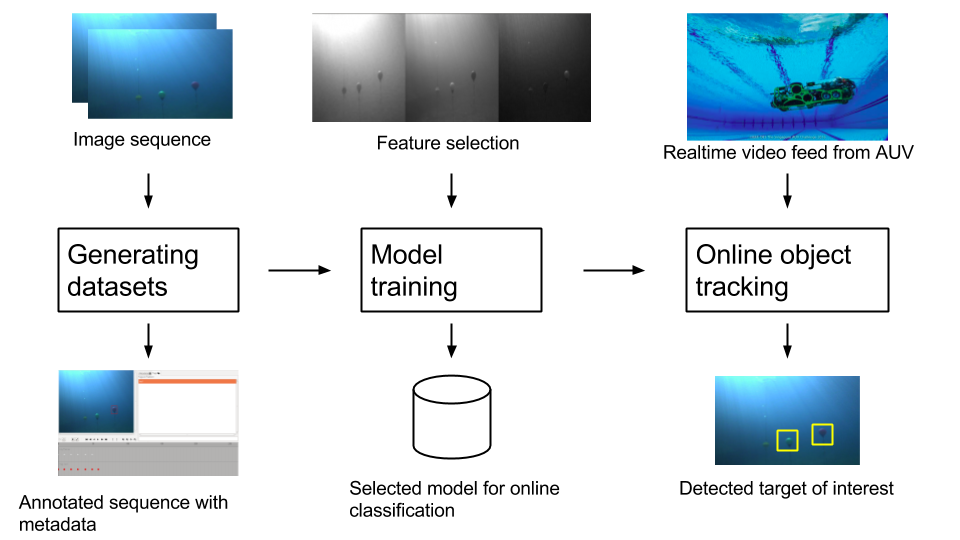
\includegraphics[width=0.8\textwidth, height=0.3\textheight]{method.png}
  \caption{Main methodology}
  \label{fig:main_methodology}
\end{figure}

\subsection{Generating datasets}

\begin{figure}[H]
\centering
  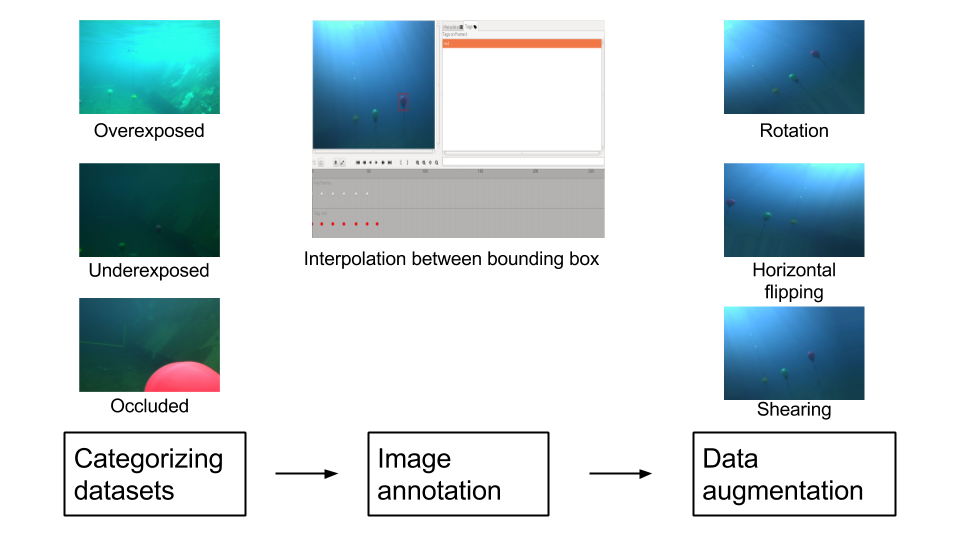
\includegraphics[width=0.8\textwidth, height=0.3\textheight]{dataset_method.png}
  \caption{Dataset generation methodology}
  \label{fig:dataset_methodology}
\end{figure}

\textbf{Data analysis} is performed on all images to further categorize them into
different datasets according to various criteria such degree of haze, existence
of shadow, illuminations and color cast. Each dataset will be tagged with
metadata generated from the analysis. Next, \textbf{video annotation} is
conducted using \textit{Mean-Shift} tracker on preprocessed images to generate
ground truth that will be used for training and validation. To prevent
overfitting and help the model generalize better, data augmentation via
horizontal flipping, scaling, rotating, shifting and color jittering is
performed with the aid of \href{https://keras.io/preprocessing/image/}{Keras
  preprocessing module}.

\subsection{Model Learning}

\begin{figure}[H]
\centering
  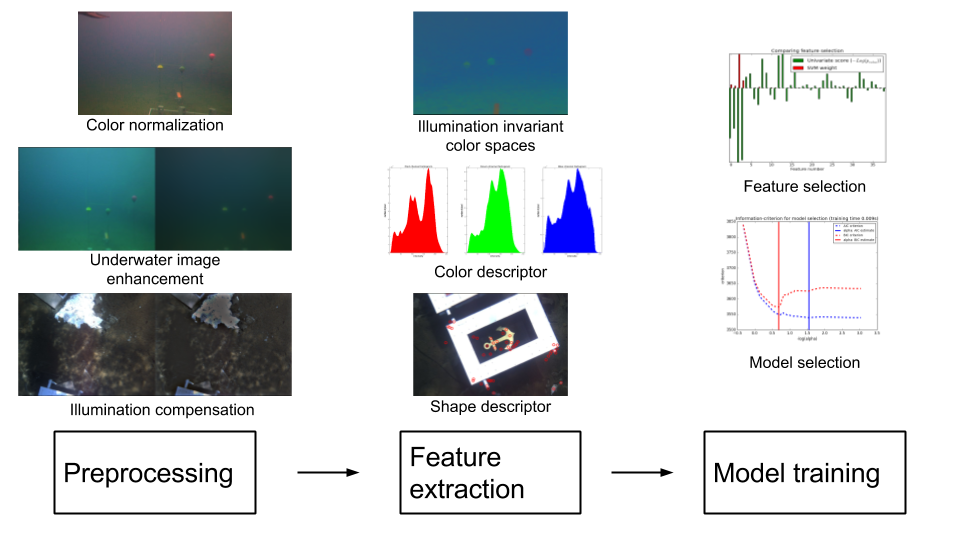
\includegraphics[width=0.8\textwidth, height=0.3\textheight]{training_method.png}
  \caption{Model learning methodology}
  \label{fig:training_methodology}
\end{figure}

To improve discriminability of objects from background in undewater setting,
\textbf{preprocessing} steps are taken such as color normalization, illumination
compensation and image enhancement. Moving on, different type of features are
extracted from various color spaces that will be used in object classification.
Using the validation set, \textbf{feature selection}, \textbf{model selection}
and \textbf{hyperparameters optimization} are executed to determine the most
optimal combination of algorithm-parameters pair for a particular object class.

\subsection{Online object detection and tracking}

\begin{figure}[H]
\centering
  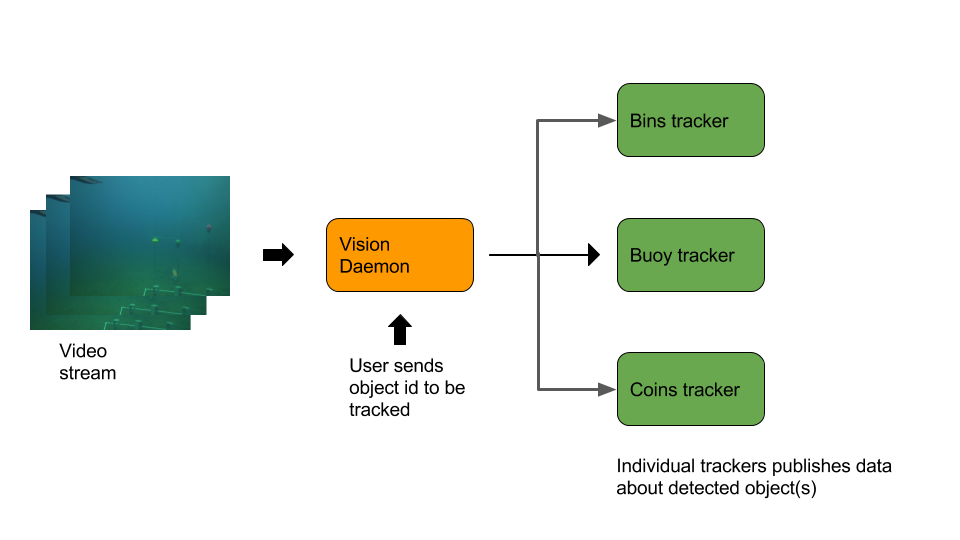
\includegraphics[width=0.8\textwidth, height=0.3\textheight]{tracking_method.png}
  \caption{Object tracking methodology}
  \label{fig:tracking_methodology}
\end{figure}

The next phase involves real-time \textbf{object proposals} adopting a)
superpixel-based clustering and b) edge detection. \textbf{Object classifier}
will rank these candidates according to classfication score. Tracking is
performed using a simple nearest neigbour approach and a new tracker will be
initialized after losing track of the target for 10 frames.

%%%%%%%%%%%%%%%%%%%%%%%%%%%%%%%%%%%%%%%%%%%%%%%%%%%%%%%%%%%%%%%%%%%%%%%%%%%%%%%
% Chapter 4: Preprocessing
%%%%%%%%%%%%%%%%%%%%%%%%%%%%%%%%%%%%%%%%%%%%%%%%%%%%%%%%%%%%%%%%%%%%%%%%%%%%%%%

\chapter{Preprocessing}

In this section, we will look into detail the preprocessing steps that are
applied to each image. 

%%%%%%%%%%%%%%%%%%%%%%%%%%%%%%%%%%%%%%%%%%%%%%%%%%%%%%%%%%%%%%%%%%%%%%%%%%%%%%%
% Chapter 6: Object Proposals
%%%%%%%%%%%%%%%%%%%%%%%%%%%%%%%%%%%%%%%%%%%%%%%%%%%%%%%%%%%%%%%%%%%%%%%%%%%%%%%

\chapter{Object Proposals}

%%%%%%%%%%%%%%%%%%%%%%%%%%%%%%%%%%%%%%%%%%%%%%%%%%%%%%%%%%%%%%%%%%%%%%%%%%%%%%%
% Chapter 7: Feature Design
%%%%%%%%%%%%%%%%%%%%%%%%%%%%%%%%%%%%%%%%%%%%%%%%%%%%%%%%%%%%%%%%%%%%%%%%%%%%%%%

\chapter{Feature Design}

%%%%%%%%%%%%%%%%%%%%%%%%%%%%%%%%%%%%%%%%%%%%%%%%%%%%%%%%%%%%%%%%%%%%%%%%%%%%%%%
% Chapter 8: Model
%%%%%%%%%%%%%%%%%%%%%%%%%%%%%%%%%%%%%%%%%%%%%%%%%%%%%%%%%%%%%%%%%%%%%%%%%%%%%%%

\chapter{Model}

%%%%%%%%%%%%%%%%%%%%%%%%%%%%%%%%%%%%%%%%%%%%%%%%%%%%%%%%%%%%%%%%%%%%%%%%%%%%%%%
% Chapter 9: Object Tracking
%%%%%%%%%%%%%%%%%%%%%%%%%%%%%%%%%%%%%%%%%%%%%%%%%%%%%%%%%%%%%%%%%%%%%%%%%%%%%%%

\chapter{Object Tracking}

%%%%%%%%%%%%%%%%%%%%%%%%%%%%%%%%%%%%%%%%%%%%%%%%%%%%%%%%%%%%%%%%%%%%%%%%%%%%%%%
% Chapter 10: Training
%%%%%%%%%%%%%%%%%%%%%%%%%%%%%%%%%%%%%%%%%%%%%%%%%%%%%%%%%%%%%%%%%%%%%%%%%%%%%%%

\chapter{Training Scheme}

%%%%%%%%%%%%%%%%%%%%%%%%%%%%%%%%%%%%%%%%%%%%%%%%%%%%%%%%%%%%%%%%%%%%%%%%%%%%%%%
% Chapter 11: Automatic machine learning
%%%%%%%%%%%%%%%%%%%%%%%%%%%%%%%%%%%%%%%%%%%%%%%%%%%%%%%%%%%%%%%%%%%%%%%%%%%%%%%

\chapter{Automatic machine learning}

%%%%%%%%%%%%%%%%%%%%%%%%%%%%%%%%%%%%%%%%%%%%%%%%%%%%%%%%%%%%%%%%%%%%%%%%%%%%%%%
% Chapter 12: Experimental results
%%%%%%%%%%%%%%%%%%%%%%%%%%%%%%%%%%%%%%%%%%%%%%%%%%%%%%%%%%%%%%%%%%%%%%%%%%%%%%%

\chapter{Experimental results}

\bibliographystyle{socreport}
\bibliography{fyp}{}

%%% End document
\end{document}
